\documentclass{standalone}

\usepackage{tikz}
\usetikzlibrary{calc}
\usetikzlibrary{math}
\usepackage{mathtools}

\DeclareMathOperator{\facemap}{d}

\begin{document}
  %noformat{
  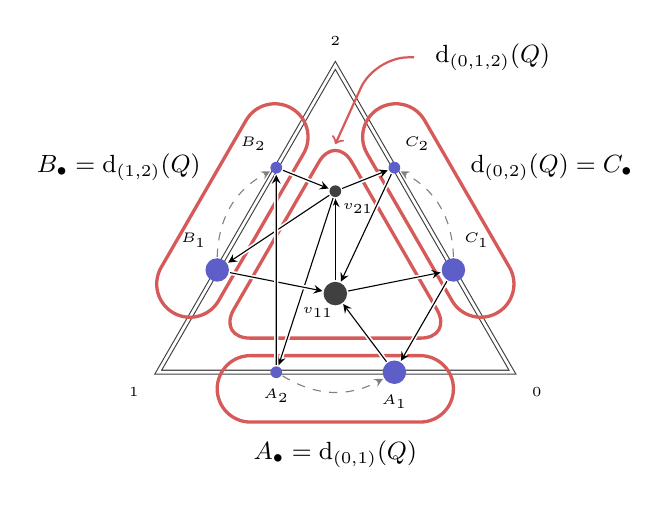
\begin{tikzpicture}
    \tikzstyle{v1} = [circle, outer xsep=0.5pt, fill, inner sep=1.5pt]
    \tikzstyle{v2} = [circle, outer xsep=0.5pt, fill, inner sep=3.0pt]
    \tikzstyle{unf} = [color=darkgray]
    \tikzstyle{frz} = [color=blue!60!darkgray!70]
    \tikzstyle{e} = [->, >={stealth}, preaction={draw=white, -, ultra thick}]
    \tikzstyle{te} = [color=darkgray, double distance=1pt]
    \tikzstyle{h} = [dashed, color=gray, ->, >={stealth}]

    \tikzset{font=\tiny}

    \tikzmath{
      \radius = 1.5*1.7321;
      \blobrad = \radius * 2/3;
      \sidelength = \radius * sin(120) / sin(30);
      \sidestep = \sidelength / 3;
    }

    \node[minimum size=5pt, label={330:{$0$}}] (l_0) at (330:\radius) {};
    \node[minimum size=5pt, label={ 90:{$2$}}] (l_2) at ( 90:\radius) {};
    \node[minimum size=5pt, label={210:{$1$}}] (l_1) at (210:\radius) {};

    \draw[te] (l_0.center) -- (l_1.center) -- (l_2.center) -- cycle;

    \node[v2,label=270:{$A_1$}, frz] (A1) at ($ (l_0.center) + (180:1*\sidestep) $) {};
    \node[v1,label=270:{$A_2$}, frz] (A2) at ($ (l_0.center) + (180:2*\sidestep) $) {};

    \node[v2,label={[shift={(-0.22,-0.6)}]{$v_{11}$}}, unf] (v11) at ( 0.0,-0.3) {};
    \node[v1,label={[shift={( 0.29,-0.5)}]{$v_{21}$}}, unf] (v21) at ( 0.0, 1.0) {};

    \node[v2,label=95:{$B_{1}$}, frz] (B1) at ($ (l_1.center) + ( 60:1*\sidestep) $) {};
    \node[v1,label=95:{$B_{2}$}, frz] (B2) at ($ (l_1.center) + ( 60:2*\sidestep) $) {};

    \node[v1,label=85:{$C_{2}$}, frz] (C2) at ($ (l_2.center) + (300:1*\sidestep) $) {};
    \node[v2,label=85:{$C_{1}$}, frz] (C1) at ($ (l_2.center) + (300:2*\sidestep) $) {};


    \draw[color=red!70!darkgray!70, rounded corners = 12pt, very thick]
        ($ (l_0.center) + (180:\sidestep*0.5) + ( 90: 6pt) $) --
        ($ (l_1.center) + (  0:\sidestep*0.5) + ( 90: 6pt) $) --
        ($ (l_1.center) + (  0:\sidestep*0.5) + (270:18pt) $) --
        ($ (l_0.center) + (180:\sidestep*0.5) + (270:18pt) $) -- cycle;

    \draw[color=red!70!darkgray!70, rounded corners = 12pt, very thick]
        ($ (l_1.center) + ( 60:\sidestep*0.5) + (330: 6pt) $) --
        ($ (l_2.center) + (240:\sidestep*0.5) + (330: 6pt) $) --
        ($ (l_2.center) + (240:\sidestep*0.5) + (150:18pt) $) --
        ($ (l_1.center) + ( 60:\sidestep*0.5) + (150:18pt) $) -- cycle;

    \draw[color=red!70!darkgray!70, rounded corners = 12pt, very thick]
        ($ (l_2.center) + (300:\sidestep*0.5) + (210: 6pt) $) --
        ($ (l_0.center) + (120:\sidestep*0.5) + (210: 6pt) $) --
        ($ (l_0.center) + (120:\sidestep*0.5) + ( 30:18pt) $) --
        ($ (l_2.center) + (300:\sidestep*0.5) + ( 30:18pt) $) -- cycle;

    \draw[color=red!70!darkgray!70, rounded corners = 12pt, very thick]
        (330:\blobrad) -- ( 90:\blobrad) -- (210:\blobrad) -- cycle;

    \node at (270:0.9*\radius) {\small $A_{\bullet} = \facemap_{(0,1)}(Q)$};
    \node at ($ ( 30:\radius) + ( 0.5,0) $) {\small $\facemap_{(0,2)}(Q) = C_{\bullet}$};
    \node at ($ (150:\radius) + (-0.5,0) $) {\small $B_{\bullet} = \facemap_{(1,2)}(Q)$};

    \node at ( 2.0, 2.7) {\small $\facemap_{(0,1,2)}(Q)$};
    \draw[->, color=red!70!darkgray!70, rounded corners=12pt, thick]
        (1.0, 2.7) --
        (0.5, 2.7) --
        ($ (l_2) + (270:1.0) $);

    \draw[h] (A2) to[bend right] (A1);
    \draw[h] (B1) to[bend left] (B2);
    \draw[h] (C1) to[bend right] (C2);

    \draw[e] (v11) -- (v21);
    \draw[e] (v11) -- (C1);
    \draw[e] (v21) -- (B1);
    \draw[e] (v21) -- (C2);
    \draw[e] (v21) -- (A2);
    \draw[e] (B1) -- (v11);
    \draw[e] (B2) -- (v21);
    \draw[e] (C1) -- (A1);
    \draw[e] (C2) -- (v11);
    \draw[e] (A1) -- (v11);
    \draw[e] (A2) -- (B2);

  \end{tikzpicture}
  %}noformat
\end{document}
